\subsection{Completación cúbica tipada del ambiente regional}
\label{vi:cubo:completacion}

La completación admite una descripción conjuntista que hace explícita su
operación. Sea \(E_9\) el conjunto de las nueve clases residuales, representadas
positivamente por \(1,\ldots,9\), y sea \(\ast\) un elemento adicional.
El símbolo \(\ast\) es distinto de la clase nula, ya representada por \(9\).
En consecuencia, la ampliación de \(E_9\) a
\(\widehat E=E_9\sqcup\{\ast\}\) aumenta el cardinal de nueve a diez
sin modificar la identificación modular interna. La completación cúbica es
\(\widehat C=\widehat E^3\), y el cubo inicial es \(C=E_9^3\).

El ambiente regional ya construido por \(\Psi\) en
\eqref{eq:psi-catalogo}, cuyo censo exacto establece la
Proposición~\ref{vi:reg:censo}, es \(\FF_3^6\). Para tipar su residencia
en el cubo inicial, escribimos \([a]_3\in\{0,1,2\}\)
para el representante de \(a\in\FF_3\) y fijamos la biyección
\[
 \eta:\FF_3^2\longrightarrow E_9,
 \qquad \eta(a,b)=1+3[a]_3+[b]_3.
\]
El agrupamiento por pares
\begin{equation}
 \beta(w_1,\ldots,w_6)=
 \bigl(\eta(w_1,w_2),\eta(w_3,w_4),\eta(w_5,w_6)\bigr)
 \label{vi:cubo:beta}
\end{equation}
es, por tanto, una biyección \(\FF_3^6\to E_9^3=S_0\). En particular,
las \(243\) palabras producidas por el censo anterior residen en el cuerpo
inicial de \(729\) posiciones; ni \(\eta\) ni \(\beta\) seleccionan una
región, una especie física o un valor metrológico. La selección regional
es una etapa posterior y distinta, demostrada en la
Proposición~\ref{vi:reg:seleccion}. La igualdad numérica
\(|\operatorname{im}\Psi|=|S_1|=243\) no identifica ambos conjuntos:
\(\beta(\operatorname{im}\Psi)\) es un subconjunto de \(S_0\), mientras
que \(S_1\) pertenece a la corona de ampliación.

\subsubsection{Diferencia de umbral y composición de coronas}
\label{vi:cubo:mg07:umbral}

La ampliación de una célula discreta conserva todos los estratos que
aparecen al aumentar su tamaño en una unidad. La diferencia de umbral
expresa esa operación sobre el lector de cardinales y permite seguir
su comportamiento bajo suma y producto antes de introducir una
realización métrica.

\begin{definition}[Diferencia de umbral]
Sea \(R\) un anillo conmutativo con unidad y sea
\(f:\mathbb Z_{\geq0}\to R\). Definimos
\begin{equation}
 (D_\#f)(n)=f(n+1)-f(n).
 \label{vi:cubo:mg07:definicion}
\end{equation}
Para un lector entero de células finitas anidadas, esta diferencia
registra el cardinal de la corona incorporada en el paso \(n\to n+1\).
\end{definition}

\begin{proposition}[Aditividad y ley exacta de producto]
Para \(f,g:\mathbb Z_{\geq0}\to R\), se cumplen
\begin{align}
 D_\#(f+g)(n)&=D_\#f(n)+D_\#g(n),
 \label{vi:cubo:mg07:aditividad}\\
 D_\#(fg)(n)&=f(n+1)D_\#g(n)+g(n)D_\#f(n)
 \label{vi:cubo:mg07:producto-desplazado}\\
 &=f(n)D_\#g(n)+g(n)D_\#f(n)
   +D_\#f(n)D_\#g(n).
 \label{vi:cubo:mg07:producto}
\end{align}
\end{proposition}

\begin{proof}
La diferencia de la suma se separa término a término. Para el producto,
introducir y sustraer \(f(n+1)g(n)\) da
\[
 \begin{split}
 f(n+1)g(n+1)-f(n)g(n)
 &=f(n+1)\bigl(g(n+1)-g(n)\bigr)\\
 &\quad+g(n)\bigl(f(n+1)-f(n)\bigr).
 \end{split}
\]
Esto prueba \eqref{vi:cubo:mg07:producto-desplazado}. La sustitución
\(f(n+1)=f(n)+D_\#f(n)\) produce
\eqref{vi:cubo:mg07:producto} con su término bilineal completo.
\end{proof}

Si \(A_n\subseteq A_{n+1}\) y \(B_n\subseteq B_{n+1}\) son
conjuntos finitos, la corona del producto se descompone en tres partes
disjuntas:
\[
 \begin{split}
 (A_{n+1}\times B_{n+1})\setminus(A_n\times B_n)
 &=\bigl(A_n\times(B_{n+1}\setminus B_n)\bigr)\\
 &\quad\sqcup\bigl((A_{n+1}\setminus A_n)\times B_n\bigr)\\
 &\quad\sqcup\bigl((A_{n+1}\setminus A_n)
                 \times(B_{n+1}\setminus B_n)\bigr).
 \end{split}
\]
Tomar cardinales da exactamente \eqref{vi:cubo:mg07:producto}. El término
bilineal cuenta las posiciones nuevas en ambos factores; su residencia
es la intersección de las dos ampliaciones, con la incidencia conservada.

\begin{proposition}[Ley binomial de la corona dimensional]
Para \(d\geq1\), sea \(f_d(n)=n^d\). Entonces
\begin{equation}
 D_\#f_d(n)=(n+1)^d-n^d
 =\sum_{k=0}^{d-1}\binom dk n^k
 =\sum_{r=1}^{d}\binom dr n^{d-r}.
 \label{vi:cubo:mg07:binomio}
\end{equation}
\end{proposition}

\begin{proof}
La expansión binomial de \((n+1)^d\) contiene \(n^d\) y los
\(d\) términos restantes de la primera suma. La sustitución
\(r=d-k\) da la segunda. En el soporte
\(\{1,\ldots,n+1\}^d\), cada posición añadida posee un conjunto
no vacío de coordenadas iguales a \(n+1\). Si ese conjunto tiene
\(r\) elementos, hay \(\binom dr\) elecciones de posiciones y
\(n^{d-r}\) elecciones de las coordenadas anteriores. Estos
estratos son disjuntos y cubren la corona; por tanto, también prueban
la fórmula mediante incidencia finita.
\end{proof}

Para \(d=3\), los tres estratos tienen cardinales \(3n^2\),
\(3n\) y \(1\). En el paso nonádico--decimal, \(n=9\), la
operación da \(243+27+1=271\); la exclusión del vértice final deja
\(270\) posiciones. La completación cúbica que sigue explicita la
unión de esta corona con las \(729\) posiciones anteriores. La ley
de umbral conserva así tanto el total como la distribución por número
de coordenadas nuevas. Las realizaciones reticulares posteriores
transportan sus incidencias mediante los mapas específicos de cada
construcción.


\begin{definition}[Estratos de codimensión combinatoria]
Para \(0\leq r\leq3\), se define
\[
 S_r=\{(x_1,x_2,x_3)\in\widehat E^3:
             \#\{j:x_j=\ast\}=r\}.
\]
El ápice de la completación es \(a_\ast=(\ast,\ast,\ast)\), y la
completación perforada es \(\widehat C^{\circ}=\widehat C\setminus\{a_\ast\}\).
\end{definition}

\begin{proposition}[Descomposición exacta de la completación]
Los estratos son disjuntos y satisfacen
\begin{align}
 \widehat C&=S_0\sqcup S_1\sqcup S_2\sqcup S_3,
 &|S_r|&=\binom3r9^{3-r},\label{vi:cubo:estratos}\\
 |\widehat C^{\circ}|&=729+243+27=999,
 &|\widehat C|&=999+1=729+271=1000.\label{vi:cubo:999}
\end{align}
La ampliación perforada contiene \(270\) elementos adicionales al cubo
inicial; la ampliación completa contiene \(271\).
\end{proposition}
\begin{proof}
Un elemento de \(S_r\) se obtiene eligiendo las \(r\) coordenadas que
contienen \(\ast\), de \(\binom3r\) maneras, y asignando a las restantes
una de las nueve clases de \(E_9\). La clasificación por el número de
coordenadas adicionales es exhaustiva y sus clases son disjuntas. El único
elemento de \(S_3\) es \(a_\ast\). Retirarlo resta una unidad al cardinal
total; restituirlo recupera el producto cartesiano completo.
\end{proof}

La expresión \emph{extrema y media razón holográfica}, abreviada EMRH en
el corpus, designa aquí esta articulación entre el cuerpo inicial, los
estratos de ampliación y la restitución unitaria. Su contenido inmediato
es la partición exacta de un producto finito y su normalización. El número
\(999\) representa un objeto determinado, la completación perforada;
\(1000\) representa su clausura por restitución del ápice. La unidad
añadida tiene, por tanto, una residencia de incidencia explícita.

\begin{figure}[htbp]
\centering
\begin{tikzpicture}[x=1cm,y=1cm,>=Stealth,font=\small]
\draw[->] (0,0)--(12.4,0);
\foreach \x/\a/\b in {0/729/{S_0},4.0/243/{S_1},7.5/27/{S_2},10.6/1/{S_3}}{
  \draw (\x,0.12)--(\x,-0.12);
  \node[above=5pt] at (\x,0) {\(\a\)};
  \node[below=5pt] at (\x,0) {\(\b\)};
}
\draw[decorate,decoration={brace,amplitude=5pt}] (0,1)--(7.7,1);
\node[above=8pt] at (3.85,1) {Completación perforada: \(999\)};
\draw[decorate,decoration={brace,mirror,amplitude=5pt}] (0,-1)--(10.8,-1);
\node[below=8pt] at (5.4,-1) {Completación íntegra: \(1000=999+1\)};
\node[align=center] at (10.6,1.5) {Ápice\\\((\ast,\ast,\ast)\)};
\end{tikzpicture}
\caption{Estratos de la completación cúbica. La disposición representa
la descomposición conjuntista, no una escala métrica. Los \(243\) elementos
de \(S_1\) son tres estratos coordenados de \(81\) elementos; los \(27\)
de \(S_2\) son tres estratos de \(9\). El ápice completa la partición.}
\label{vi:cubo:estratos-fig}
\end{figure}

% Inclusión de la figura histórica vectorial en escala de grises.
% El PDF y su fuente standalone se conservan literalmente como cubo_emrh_original.*.
\begin{figure}[htbp]
\centering
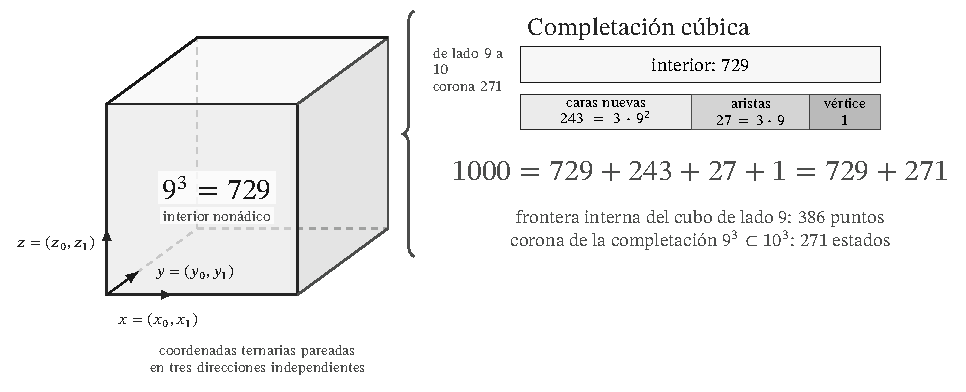
\includegraphics[width=\textwidth]{figures/cubo_emrh_original.pdf}
\caption{Representación cúbica de la ampliación de nueve a diez clases por coordenada. Los estratos \(S_1,S_2,S_3\) sitúan las incidencias añadidas en caras, aristas y ápice; sus cardinales forman la corona de \(271\) elementos. La frontera de \(386\) elementos pertenece al cubo inicial. La perspectiva geométrica complementa la partición de la figura~\ref{vi:cubo:estratos-fig}; las separaciones gráficas tienen función esquemática.}
\label{vi:cubo:completacion-3d}
\end{figure}


\subsubsection{Conservación de la unidad y compatibilidad dimensional}

La normalización no se limita a dividir una identidad aislada. En dimensión
\(d\), el producto \(\widehat E^d\) lleva la medida uniforme
\(\mu_d(\{x\})=10^{-d}\). La proyección coordenada
\(p_d:\widehat E^{d+1}\to\widehat E^d\) suprime la última coordenada.

\begin{proposition}[Compatibilidad proyectiva de las medidas normalizadas]
Para todo \(d\geq1\),
\[
 (p_d)_*\mu_{d+1}=\mu_d,
 \qquad \mu_d(\widehat E^d)=1.
\]
La masa del estrato con \(r\) coordenadas adicionales es
\(\binom dr9^{d-r}/10^d\), y la suma de las masas de todos los estratos
es uno.
\end{proposition}
\begin{proof}
Cada punto de \(\widehat E^d\) tiene diez preimágenes. Su masa total es
\(10\,10^{-(d+1)}=10^{-d}\). La igualdad para cualquier subconjunto
se obtiene sumando sobre sus puntos. La fórmula estratificada procede
del mismo recuento que \eqref{vi:cubo:estratos}; el binomio
\((9+1)^d\) da la normalización total.
\end{proof}

En dimensión tres, retirar el ápice deja masa \(999/1000\), y
restituirlo añade \(1/1000\). Renormalizar antes de la restitución
definiría otra medida: la distinción es operacionalmente relevante.
En particular, conservación de masa probabilística, conservación de los
registros de transporte y disipación termodinámica son afirmaciones con
objetos diferentes. La proposición demuestra la primera y proporciona el
soporte compatible para estudiar la segunda; la tercera requiere una
realización dinámica y energética especificada.

También permanece diferenciada la frontera geométrica interna.
Sobre el representante cartesiano \(\{1,\ldots,9\}^3\), retirar
\(\{2,\ldots,8\}^3\) deja \(386\) puntos. Esta frontera pertenece al
cubo inicial, mientras \(\widehat C\setminus C\) pertenece a su
ampliación. La completación cúbica, la expansión posicional de base mil y
la lectura de incidencia excepcional comparten datos del soporte;
sus mapas respectivos determinan qué información de esos datos utiliza
cada representación.
